This section evaluates the performance of the cached profile implementation using modern benchmark suites. The goal is to provide indicators on the performance influence and try to analyze where this performance influence comes from. Since we try to decrease warmup time and decrease the number of deoptimizations 
\section{Setup}
\label{s:perf_setup}
To provide reliable and comparable results all tests were done on a single node of the Data Center Observatory provided by ETH \cite{ethdco}.
A node features 2 8-Core AMD Opteron 6212 CPUs running at 2600 MHz with 128 GB of DDR3 RAM.
The node is running Fedora 19 and GCC 4.8.3. All JDK builds got created on the node itself.
\\\\
To compare performance the following benchmarks were used:
\begin{enumerate}
  \item \textbf{SPECjvm 2008:} A benchmark suite developed by Standard Performance Evaluation Corporation for measuring the performance of the Java Runtime Environment \cite{specjvm}.  I use version 2008 and I run a subset of 17 out of a total of 21 benchmarks. 4 are omitted due to incompatibility with openJDK 1.9.0.
  \\
  Once finished, SPECjvm prints out the number of operations per minute. This is used to compare the performance and higher is better.
  \item \textbf{Octane 2.0:} A benchmark developed by Google to measure the performance of JavaScript code found in large, real-world applications \cite{octane}. Octane runs on Nashorn, a JavaScript Engine on top of Hotspot. The version used is 2.0 and consists of 17 individual benchmarks of which 16 are used.
  \\
  Octane gives each benchmark a score reflecting the performance, the higher the score, the better the performance.
\end{enumerate}
The benchmarking process was automated using a number of self-written python scripts. The graphs in this chapter always show the arithmetic mean of 50 runs and the error bars display the 95\% confidence intervals.

\section{Benchmark performance}
\label{s:perf_benchmark}
The main goal of cached profiles is to improve the startup performance of the JVM. Having a rich profile from an earlier execution will allow the JIT compiler to use a highly optimized version right from the beginning.
We expect the modes to produce different results. The following list suggests reasons for these performance differences:
\begin{itemize}
  \item Some benchmarks might profit from compiling methods very early and therefore favor Mode 0.
  \item That could however result in many early compilations that overload the compilation queue resulting in worse performance. In this case Mode 1 will perform better than Mode 0.
  \item In case a cached profile can not be used (i.e. the limit of 10 deoptimizations was reached) the JVM needs to use freshly generated profiles. In case the thresholds were lowered (Mode 0) this compilation might have happened very early and only very incomplete profiles were available. This effect is less a problem when Mode 1 is used.
  \item Mode 2 keeps the steps of the original tiered compilation and is considered the most conservative mode. It puts the same load on the compile queue than the baseline version.
\end{itemize}
I will start by looking at SPECjvm since it offers ways to focus on the warmup. An individual description of each benchmark being used can be found in Appendix \ref{a:specjvm_benchmark}.
\subsection{SPECjvm warmup performance}
\label{s:perf_specjvm_warmup}
The longer a program is running the less impact a faster warmup has. Considering most benchmarks include a warmup phase which does not count towards the final score simply running the complete benchmark suite is not an option.
Instead I limited SPECjvm to 1 single operation which, depending on the benchmark take around 6 to 40 seconds.
Additionally, the JVM gets restarted between each single benchmark to prevent methods shared between benchmarks being compiled already.
\\\\
I run each benchmark with all cached profiling features disabled. This run is called the \textit{baseline} and displays the current openJDK 1.9.0 performance.    
\\\\ 
I then use a single benchmark run where I dump the profiles to disk. This run is not limited to a single operation and instead uses the default values of the benchmark. By default the benchmark is limited by time and runs for about 6 minutes. The idea is that these profiles include information that are usually not available during warmup and result in less deoptimizations and better code quality.
\\\\
These profiles are then used in 3 individual runs using the introduced \texttt{-XX:CacheProfiles} flag. Each run is using one of the 3 different CacheProfilesModes.
\begin{figure}[ht]
  \begin{center}
    \centering
    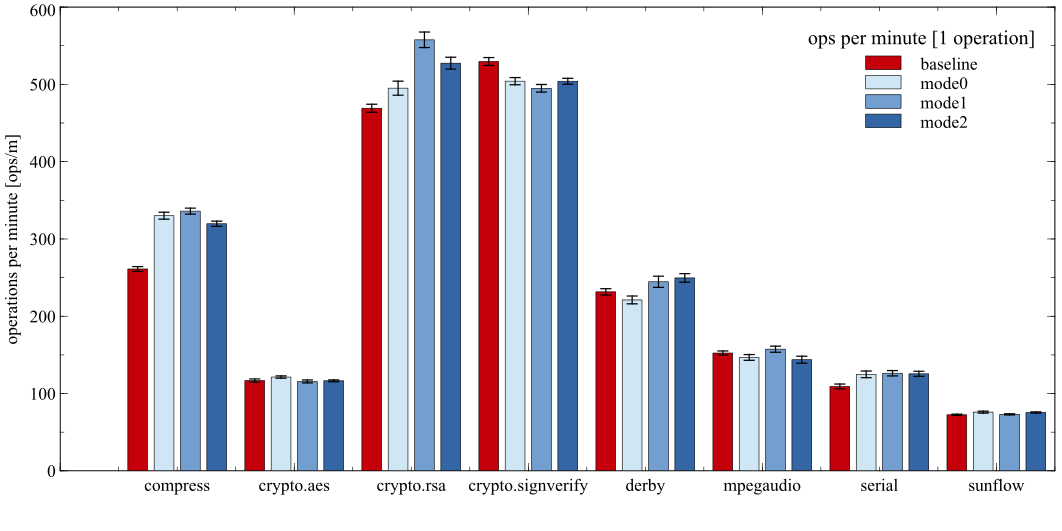
\includegraphics[width=1.0\textwidth]{figures/others_warmup.png}
    \caption{SPECjvm benchmarks on all different modes}
    \label{f:others_warmup}
  \end{center}
\end{figure}
\begin{figure}[ht]
  \begin{center}
    \centering
    \includegraphics[width=1.0\textwidth]{figures/scimark_warmup.png}
    \caption{SPECjvm scimark benchmarks on all different modes}
    \label{f:scimark_warmup}
  \end{center}
\end{figure}

\begin{figure}[ht]
  \begin{center}
    \centering
    \includegraphics[width=1.0\textwidth]{figures/all_warmup_variation.png}
    \caption{Relative performance from baseline for all SPECjvm benchmarks}
    \label{f:all_warmup_variation}
  \end{center}
\end{figure}
Figures \ref{f:others_warmup} and \ref{f:scimark_warmup} shows the number of operations per minute, measured for each benchmark individually. Note, that the operations per minute is not to be confused with the \textit{1 operation }of the benchmark itself.
Figure \ref{f:all_warmup_variation} summarizes the results by showing the relative performance compared to the baseline.
\\\\
The individual benchmarks show different effects on performance. Taking the average of all modes, we see a performance increase up to around 34\% in the compress benchmark (Mode 1) and a performance decrease of down to 20\% in scimark.sparse.large (Mode 0).
\\\\
Interestingly, the performance differences between the modes is not the same when comparing the individual benchmarks. For example in crypto.rsa Mode 0 clearly performs worst but in scimark.sparse.small it performs best.
JVM performance is known to be very hard to predict and it seems not to be different when cached profiles are used. On average the performance of the benchmark warmup is improved by 2.64\%, 3.37\%, and 2.67\% for Mode 0, Mode 1 and Mode 2.
\\\\
Between the three different modes there is no clear \textit{winner}. Each mode wins and looses in certain benchmarks against the others in terms of performance. However, in 12 out of 17 benchmarks at least one of the CacheProfileModes improves performance. 
\\\\
We will take a more detailed look at single benchmarks later in this chapter. 
\subsection{Octane performance}
\label{s:perf_octane}
Since the individual Octane benchmarks are rather short (most of them run for between 4 and 30 seconds) and there is no way to run a fixed number of iterations (without modifying the Octane source) we run the Octane benchmarks completely. We still split up the execution in the individual benchmarks to achieve many JVM restarts. The rest of the setup is identical to the SPECjvm run in Section \ref{s:perf_specjvm_warmup}.
\\\\
The absolute results are shown in Figure \ref{f:octane} and a relative comparison with the baseline in Figure \ref{f:octane_variation}.
Compared to SPECjvm the Octane performance is more scattered. The richards benchmark increases by around 50\% in Mode 0 while navierstockes decreases by around 25\% in Mode 1. In most benchmarks (9 out of 14) Mode 0 performs worst.
We assume this is related to the increased load of the compile queue and will therefore take a more detailed look at this in Section \ref{s:perf_compilequeue}. The performance of the two other modes is better in most benchmarks, but in total only 6 out of 14 benchmarks result in a performance improvement in at least one mode.

\begin{figure}[ht]
  \begin{center}
    \centering
    \includegraphics[width=1.0\textwidth]{figures/octane.png}
    \caption{Octane benchmarks on all different modes}
    \label{f:octane}
  \end{center}
\end{figure}

\begin{figure}[ht]
  \begin{center}
    \centering
    \includegraphics[width=1.0\textwidth]{figures/octane_variation.png}
    \caption{Relative performance from baseline for all Octane benchmarks}
    \label{f:octane_variation}
  \end{center}
\end{figure}


% \section{Without Intrinsics}
% \label{s:without_intrinsics}
%
% \begin{figure}[ht]
%   \begin{center}
%     \centering
%     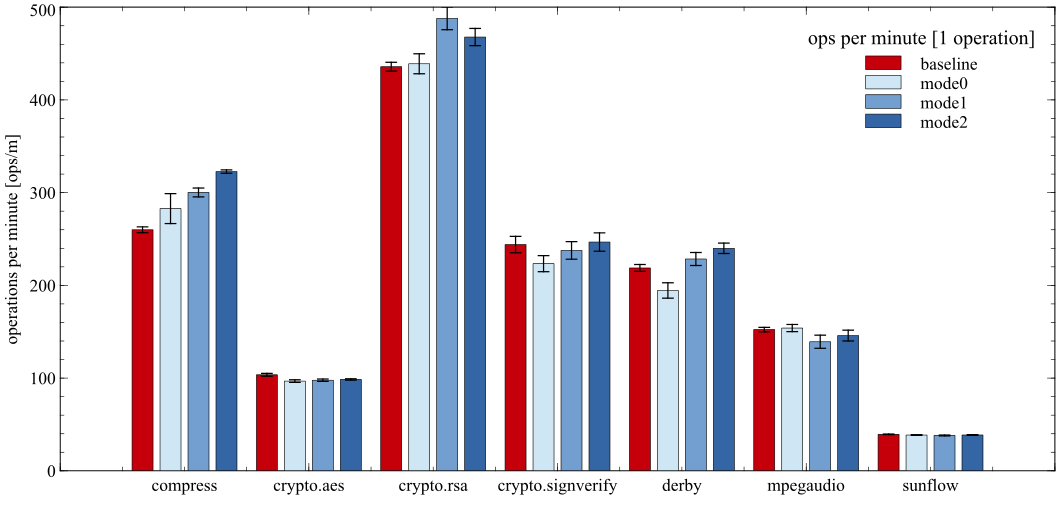
\includegraphics[width=1.0\textwidth]{figures/others_warmup_nointrinsics.png}
%     \caption{SPECjvm benchmarks on all different modes without intrinsified methods}
%     \label{f:others_warmup_nointrinsics}
%   \end{center}
% \end{figure}
%
% \begin{figure}[ht]
%   \begin{center}
%     \centering
%     \includegraphics[width=1.0\textwidth]{figures/scimark_warmup_nointrinsics.png}
%     \caption{SPECjvm scimark benchmarks on all different modes without intrinsified methods}
%     \label{f:scimark_warmup_nointrinsics}
%   \end{center}
% \end{figure}
%
%
% \begin{figure}[ht]
%   \begin{center}
%     \centering
%     \includegraphics[width=1.0\textwidth]{figures/all_warmup_nointrinsics_variation.png}
%     \caption{Relative performance from baseline for all SPECjvm benchmarks without intrinsified methods}
%     \label{f:all_warmup_nointrinsics_variation}
%   \end{center}
% \end{figure}


\section{Deoptimizations}
\label{s:perf_deoptimizations}
We are still eager to figure out where the performance increase and decrease come from.
We aim to lower the time needed for warmup by compiling methods earlier and or at lower tiers but also expect to decrease the number of deoptimizations by having more complete profiles early, which ideally results in better compiled code quality.
The total number of deoptimizations of the SPECjvm benchmarks is shown in Figure \ref{others_warmup_deopt} and Figure \ref{f:scimark_warmup_deopt}. The Octane numbers are drawn in Figure \ref{octane_deopt}.
Again, we also included graphs that show the number of deoptimizations relative to the baseline runs in Figure \ref{f:all_warmup_variation_deopt} and Figure \ref{f:octane_variation_deopt}.
\\\\
The measurements show, that when using Mode 1 or Mode 2, we are able to reduce the deoptimizations significantly in all benchmarks except one (gameboy). In Mode 0 there is a clear difference between SPECjvm and Octane. While in SPECjvm the number of deoptimizations is similar to the other modes, in Octane Mode 0 on average increases the number by 30\%. Mode 0 also had the worst performance for Octane and we assume the amount of deoptimizations to be one of the reasons for that regression.
\\\\
And while a low deoptimization number is a good indication of the increased code quality for methods being compiled with cached profiles we could not find a direct correlation between number of deoptimizations and the result on the performance.
\begin{figure}[ht]
  \begin{center}
    \centering
    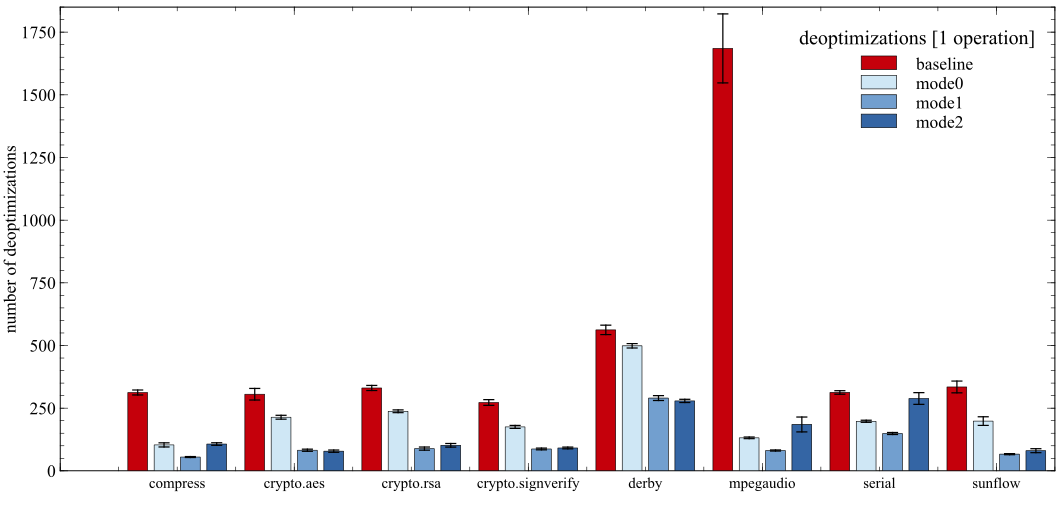
\includegraphics[width=1.0\textwidth]{figures/others_warmup_deopt.png}
    \caption{SPECjvm deoptimizations of all modes}
    \label{f:others_warmup_deopt}
  \end{center}
\end{figure}

\begin{figure}[ht]
  \begin{center}
    \centering
    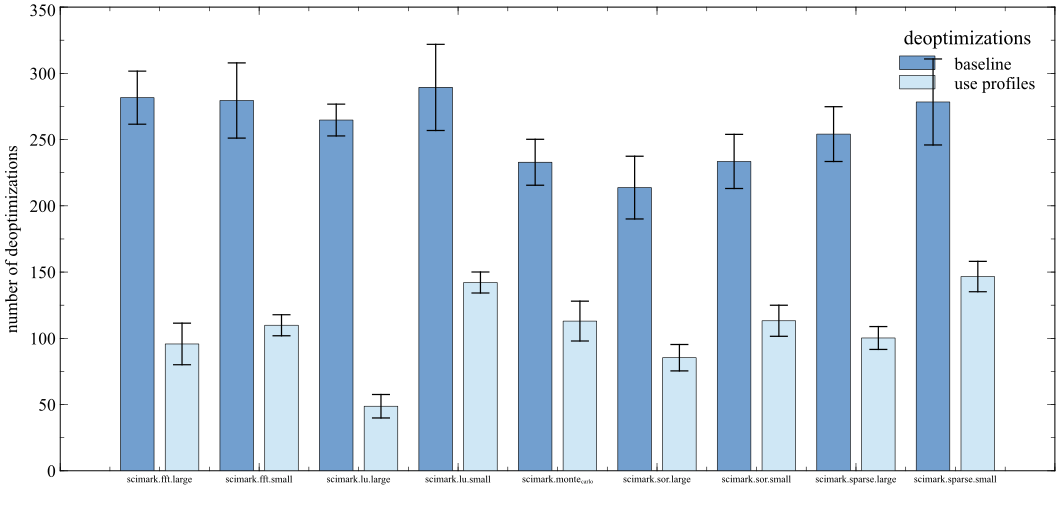
\includegraphics[width=1.0\textwidth]{figures/scimark_warmup_deopt.png}
    \caption{SPECjvm scimark deoptimizations of all modes}
    \label{f:scimark_warmup_deopt}
  \end{center}
\end{figure}

\begin{figure}[ht]
  \begin{center}
    \centering
    \includegraphics[width=1.0\textwidth]{figures/all_warmup_variation_deopt.png}
    \caption{Relative deoptimizations from baseline for all SPECjvm benchmarks}
    \label{f:all_warmup_variation_deopt}
  \end{center}
\end{figure}

\begin{figure}[ht]
  \begin{center}
    \centering
    \includegraphics[width=1.0\textwidth]{figures/octane_deopt.png}
    \caption{Octane deoptimizations of all modes} 
    \label{f:octane_deopt}
  \end{center}
\end{figure}



\begin{figure}[ht]
  \begin{center}
    \centering
    \includegraphics[width=1.0\textwidth]{figures/octane_variation_deopt.png}
    \caption{Relative deoptimizations from baseline for all Octane benchmarks}
    \label{f:octane_variation_deopt}
  \end{center}
\end{figure}

\clearpage
\section{Effect on compile queue}
\label{s:perf_compilequeue}

% --------------------------- Octane Richards Queue ------------------
\begin{figure}[ht]
  \begin{center}
    \centering
    \includegraphics[width=0.9\textwidth]{figures/octane_queue_richards_separate_c1.png}
    \caption{C1 Compile queue size over time Octane Richards benchmark}
    \label{f:octane_queue_richards_separate_c1}
  \end{center}
\end{figure}
\begin{figure}[ht]
  \begin{center}
    \centering
    \includegraphics[width=0.9\textwidth]{figures/octane_queue_richards_separate_c2.png}
    \caption{C2 Compile queue size over time Octane Richards benchmark}
    \label{f:octane_queue_richards_separate_c2}
  \end{center}
\end{figure}
% --------------------------- Octane EarleyBoyer Queue ------------------
\begin{figure}[ht]
  \begin{center}
    \centering
    \includegraphics[width=1.0\textwidth]{figures/octane_queue_earleyboyer_separate_c1.png}
    \caption{C1 Compile queue size over time Octane EarleyBoyer benchmark}
    \label{f:octane_queue_earleyboyer_separate_c1}
  \end{center}
\end{figure}
\begin{figure}[ht]
  \begin{center}
    \centering
    \includegraphics[width=1.0\textwidth]{figures/octane_queue_earleyboyer_separate_c2.png}
    \caption{C2 Compile queue size over time Octane EarleyBoyer benchmark}
    \label{f:octane_queue_earleyboyer_separate_c2}
  \end{center}
\end{figure}
% --------------------------- Octane NavierStokes Queue ------------------
\begin{figure}[ht]
  \begin{center}
    \centering
    \includegraphics[width=1.0\textwidth]{figures/octane_queue_navierstokes_separate_c1.png}
    \caption{C1 Compile queue size over time Octane NavierStokes benchmark}
    \label{f:octane_queue_navierstokes_separate_c1}
  \end{center}
\end{figure}
\begin{figure}[ht]
  \begin{center}
    \centering
    \includegraphics[width=1.0\textwidth]{figures/octane_queue_navierstokes_separate_c2.png}
    \caption{C2 Compile queue size over time Octane NavierStokes benchmark}
    \label{f:octane_queue_navierstokes_separate_c2}
  \end{center}
\end{figure}
% --------------------------- Octane DeltaBlue Queue ------------------
\begin{figure}[ht]
  \begin{center}
    \centering
    \includegraphics[width=1.0\textwidth]{figures/octane_queue_deltablue_separate_c1.png}
    \caption{C1 Compile queue size over time Octane DeltaBlue benchmark}
    \label{f:octane_queue_deltablue_separate_c1}
  \end{center}
\end{figure}
\begin{figure}[ht]
  \begin{center}
    \centering
    \includegraphics[width=1.0\textwidth]{figures/octane_queue_deltablue_separate_c2.png}
    \caption{C2 Compile queue size over time Octane DeltaBlue benchmark}
    \label{f:octane_queue_deltablue_separate_c2}
  \end{center}
\end{figure}
% --------------------------- SPECjvm compress Queue ------------------
\begin{figure}[ht]
  \begin{center}
    \centering
    \includegraphics[width=1.0\textwidth]{figures/spec_queue_compress_separate_c1.png}
    \caption{C1 Compile queue size over time SPECjvm compress benchmark}
    \label{f:spec_queue_compress_separate_c1}
  \end{center}
\end{figure}
\begin{figure}[ht]
  \begin{center}
    \centering
    \includegraphics[width=1.0\textwidth]{figures/spec_queue_compress_separate_c2.png}
    \caption{C2 Compile queue size over time SPECjvm compress benchmark}
    \label{f:spec_queue_compress_separate_c2}
  \end{center}
\end{figure}
% --------------------------- SPECjvm scimark.sparse.large Queue ------------------
\begin{figure}[ht]
  \begin{center}
    \centering
    \includegraphics[width=1.0\textwidth]{figures/spec_queue_scirmarksparselarge_separate_c1.png}
    \caption{C1 Compile queue size over time SPECjvm scimark.sparse.large benchmark}
    \label{f:spec_queue_scirmarksparselarge_separate_c1}
  \end{center}
\end{figure}
\begin{figure}[ht]
  \begin{center}
    \centering
    \includegraphics[width=1.0\textwidth]{figures/spec_queue_scirmarksparselarge_separate_c2.png}
    \caption{C2 Compile queue size over time SPECjvm scimark.sparse.large benchmark}
    \label{f:spec_queue_scirmarksparselarge_separate_c2}
  \end{center}
\end{figure}
% --------------------------- Queue Total ------------------
\begin{figure}[ht]
  \begin{center}
    \centering
    \includegraphics[width=1.0\textwidth]{figures/queue_total.png}
    \caption{Number of compilations for some specJVM and octane benchmarks}
    \label{f:queue_total}
  \end{center}
\end{figure}

\clearpage

% --------------------------- Compilation cake Richards ------------------
\begin{figure}[ht]
  \begin{center}
    \centering
    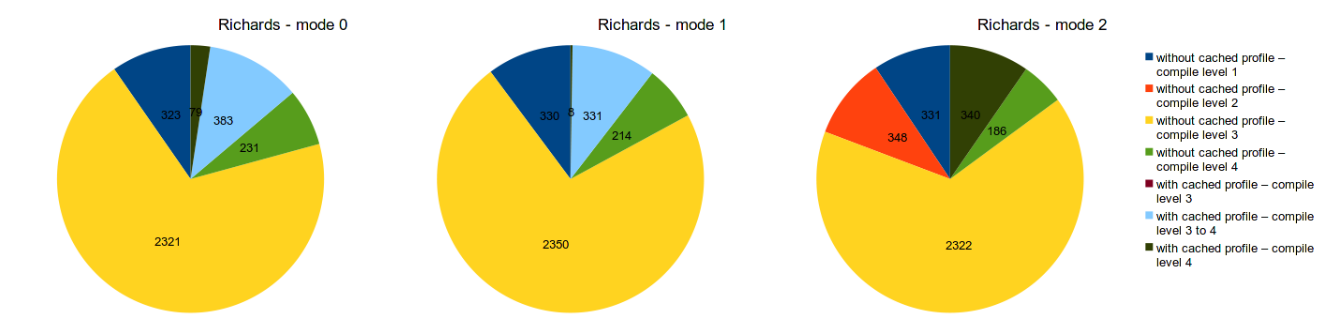
\includegraphics[width=1.0\textwidth]{figures/richards_compilations.png}
    \caption{Ratio of compilations Octane Richards benchmark}
    \label{f:richards_compilations}
  \end{center}
\end{figure}
% --------------------------- Compilation cake Richards ------------------
\begin{figure}[ht]
  \begin{center}
    \centering
    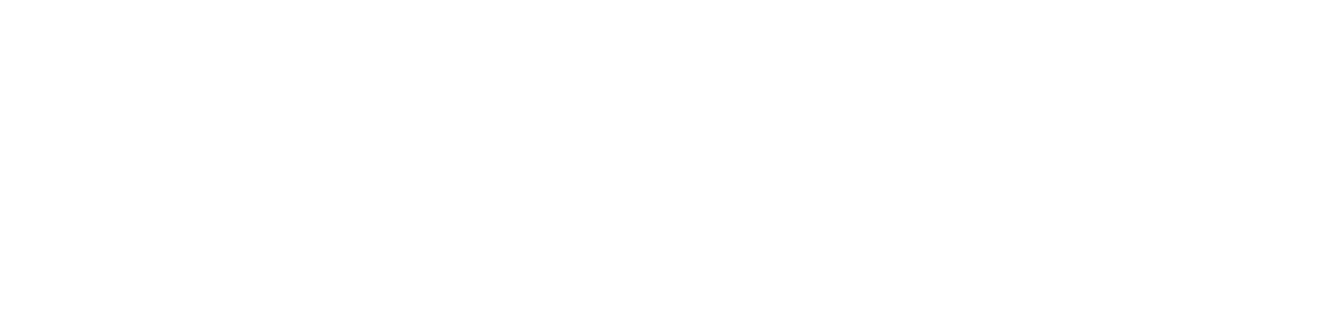
\includegraphics[width=1.0\textwidth]{figures/deltablue_compilations.png}
    \caption{Ratio of compilations Octane DeltaBlue benchmark}
    \label{f:deltablue_compilations}
  \end{center}
\end{figure}
% --------------------------- Compilation cake Richards ------------------
\begin{figure}[ht]
  \begin{center}
    \centering
    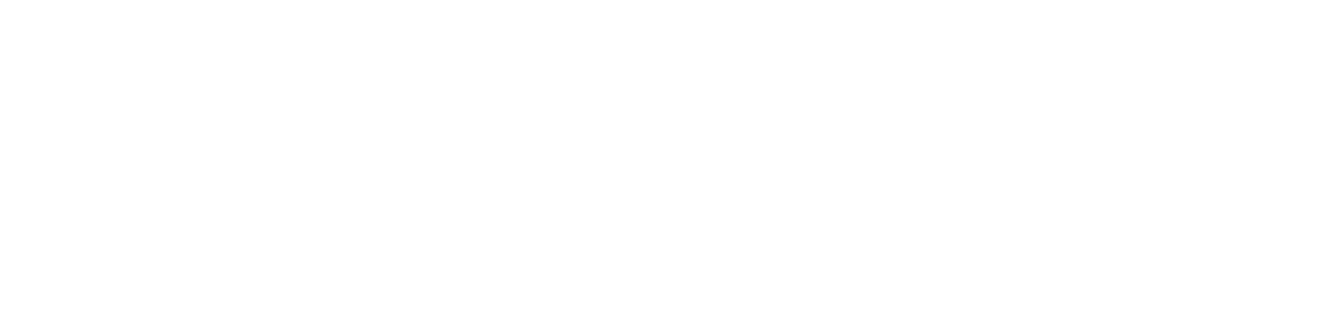
\includegraphics[width=1.0\textwidth]{figures/earleyboyer_compilations.png}
    \caption{Ratio of compilations Octane EarleyBoyer benchmark}
    \label{f:earleyboyer_compilations}
  \end{center}
\end{figure}
% --------------------------- Compilation cake Richards ------------------
\begin{figure}[ht]
  \begin{center}
    \centering
    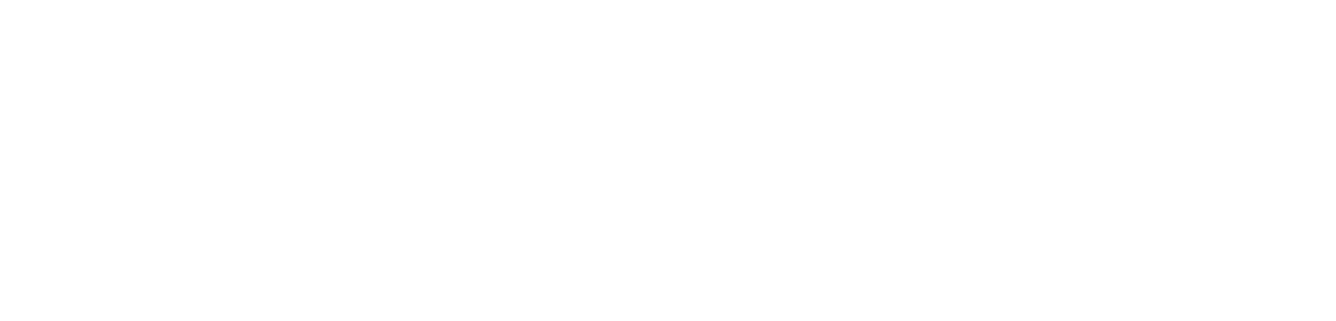
\includegraphics[width=1.0\textwidth]{figures/navierstokes_compilations.png}
    \caption{Ratio of compilations Octane NavierStokes benchmark}
    \label{f:navierstokes_compilations}
  \end{center}
\end{figure}
% --------------------------- Compilation cake compress ------------------
\begin{figure}[ht]
  \begin{center}
    \centering
    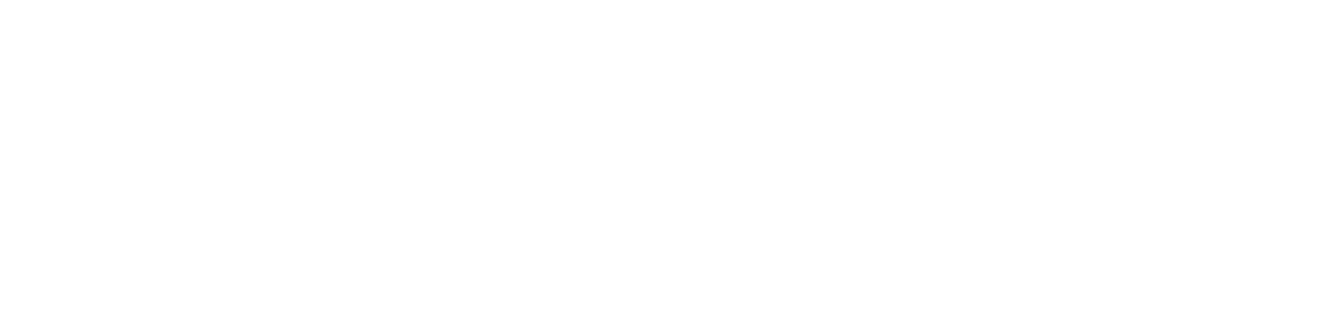
\includegraphics[width=1.0\textwidth]{figures/compress_compilations.png}
    \caption{Ratio of compilations SPECjvm compress benchmark}
    \label{f:compress_compilations}
  \end{center}
\end{figure}
% --------------------------- Compilation cake sparse.large ------------------
\begin{figure}[ht]
  \begin{center}
    \centering
    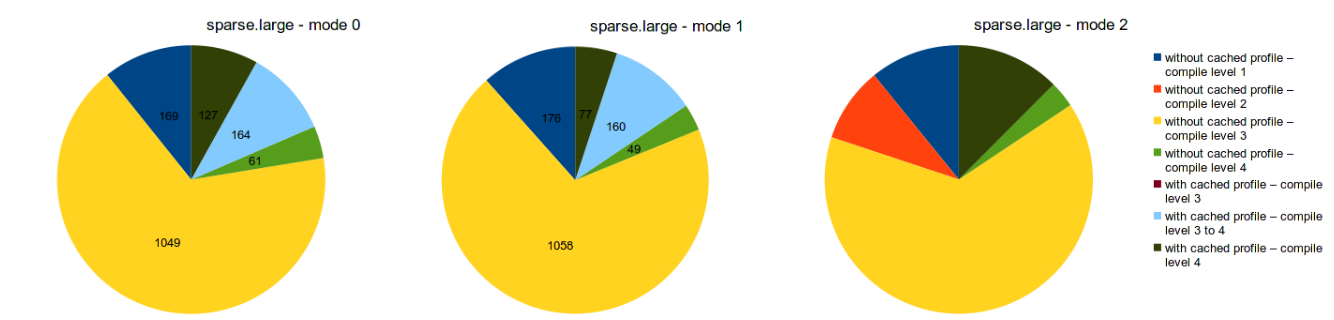
\includegraphics[width=1.0\textwidth]{figures/sparselarge_compilations.png}
    \caption{Ratio of compilations SPECjvm sparse.large benchmark}
    \label{f:sparselarge_compilations}
  \end{center}
\end{figure}
